%%%%%%%%%%%%%%%%%%%%%%%%%
% PACKAGES              %
%%%%%%%%%%%%%%%%%%%%%%%%%
\documentclass[]{report} % book|article|…

\usepackage[utf8x]{inputenc}    % accents
\usepackage{geometry}           % marges
\usepackage[francais]{babel}    % langue
\usepackage{graphicx}           % images
\usepackage{verbatim}           % texte préformaté
\usepackage{fancyhdr}           % fancy
\usepackage{filecontents}       % write file directly
\usepackage{csvsimple}          % csv reader
\usepackage{lastpage}	        % get number of last page
\usepackage{listings}           % source code 
\usepackage{url}                % clickable urls 
\usepackage{float}              % exact placing of figures

% packages for graphics
\usepackage{fancybox}         
\usepackage{pgfplots}        
\usepackage{pgfplotstable}
\usepgfplotslibrary{dateplot}
\usepackage{pgfplots}

\definecolor{Gene0}{RGB}{250, 164, 1}
\definecolor{Gene1}{RGB}{128, 0, 128}
\definecolor{Gene2}{RGB}{255, 0, 0}
\definecolor{Gene3}{RGB}{58, 242, 75}
\definecolor{Gene4}{RGB}{8, 81, 156}
\definecolor{Diversity}{RGB}{0, 0, 0}

\pgfplotscreateplotcyclelist{list}{
        {Gene0},
        {Gene1},
        {Gene2},
        {Gene3},
        {Gene4},
        {Diversity}
}



%%%%%%%%%%%%%%%%%%%%%%%%%
% PRÉAMBULE             %
%%%%%%%%%%%%%%%%%%%%%%%%%
\title{Genomat\\PRJ project Report}
\author{Ostiane D'AUGUSTIN and Lucas BOURNEUF}
% laisser vide pour date de compilation
\date{} 

% FORMAT PAGES         
\pagestyle{fancy} % nom du rendu (définit les lignes suivantes)
        \lhead{M1 BIG} % left head
        \chead{} % center head
        \rhead{2014/2015} % right head
        \lfoot{} % left foot
        \cfoot{\thepage/\pageref{LastPage}} % center foot
        \rfoot{} % right foot






%%%%%%%%%%%%%%%%%%%%%%%%%
% BEGIN                 %
%%%%%%%%%%%%%%%%%%%%%%%%%
\begin{document}
        \maketitle % page de titre




%%%%%%%%%%%%%%%%%%%%%%%%%
% SECTION               %
%%%%%%%%%%%%%%%%%%%%%%%%%
\section*{Introduction}
	\paragraph*{}
	The aim of this project is to implement a genetic algorithm which will bring out the connexions between different genes, 
        their regulation networks, and some properties linked to, as well as their resistance to genes knock-out (KO).
	\paragraph*{}
	We will study a famous genes network example, which has been highlighted by Wagner. Wagner's genes network is an artificial genes network calculation model. 
        It has explained all the development and evolution process of genetic regulation networks. It has been first developed by Andreas Wagner in 1996, 
        and then used by several research teams in order to study genes network evolution, genes expression, etc.
	\paragraph*{}
	We will simulate \textit{in silico} a population's evolution over many generations. Each individual is characterized by his genotype 
        (that is to say, its genes network). 
        Individuals will be submit to an evolutive process by the intermediary of their genes networks.




%%%%%%%%%%%%%%%%%%%%%%%%%
% SECTION               %
%%%%%%%%%%%%%%%%%%%%%%%%%
\section*{Project organization}
	\paragraph*{}
        The project follows a Python-like packaging, with the main program launchable as a package. (\textit{python -m genomat})
        Many parameters can be sended through command-line arguments, or configuration file.
        Outputs are mainly in \textsc{csv format}. (notabily those provided for statistics)

	\paragraph*{}
        A second and incomplete implementation of Genomat is available under the name of \textit{genomat\_func}. 
        This implementation is only here as a proof of concept that use a functionnal approach.

	\paragraph*{}
        Used technologies :
        \begin{description}
                \item[python] as the main language (version 3.4);
                \item[docopt] as command-line arguments parser;
                \item[doctest] for unit tests in some docstrings (see \textsc{unittests.py} file);
                \item[numpy] for manage matrix (and notabily multiplications) until Python 3.5 interpreter is available;
                \item[latex] for present report, with pgfplot module for automatic data vizualization generation;
                \item[pylint] for source code profiling and UML generation;
                \item[make] for automatize simulations, tests, etc;
        \end{description}



%%%%%%%%%%%%%%%%%%%%%%%%%
% SECTION               %
%%%%%%%%%%%%%%%%%%%%%%%%%
\section*{Source code architecture}
	\paragraph*{}
        Genomat is cut in modules as shown in Figure~\ref{fig:umldiag}, and described below.
        \begin{description}
                \item[main] implements a simple and efficient interface that allow command-line arguments;
                \item[config] management of configurations : files, options, flags, serialization;
                \item[gene network] definition of an individual, encapsulation of numpy matrix system;
                \item[population] a list of individuals that provides many data access and call stats modules as an observer;
                \item[stats] observer of population that tests it and generate, if asked, data in targeted files;
                \item[progress bar] dumb and simple implementation of a progress bar, designed to be replaced later;
        \end{description}

        \begin{figure}[H] 
                \centering
                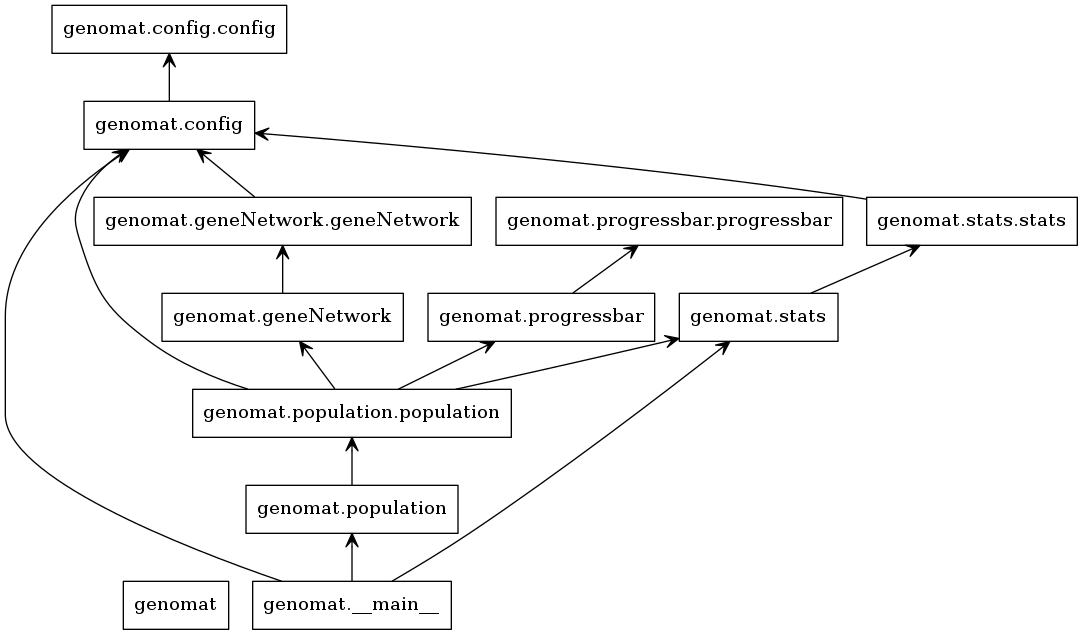
\includegraphics[width=\textwidth]{packages_genomat.png}
                \caption{Modules of Genomat architecture, without externals ones (numpy, docopt).}
                \label{fig:umldiag}
        \end{figure}




%%%%%%%%%%%%%%%%%%%%%%%%%
% SECTION               %
%%%%%%%%%%%%%%%%%%%%%%%%%
\section{Watchables}
    \paragraph*{}
    Main data generated results of gene KO, for each gene at each generation. 
    A diversity ratio is also computed at each generation.
    \paragraph*{}
     First, we tested our program with the parameters given by the subject, that is to say 200 generations with 300 individuals per generation. 
     As there was no mutation rate given, we varied it from $10^{-1}$ (that is to say, a mutation rate of 1) to $10^{-6}$. 
     We will then study the influence of the mutation rate on a random population of 300 individuals over 200 generations.
    \paragraph*{}
     With those parameters, we can notice the five genes have a similar course : their survivability ratio first fastly 
     increase from 0.7 during the fifty first generations. After this exponentianal phase, the survavibility ratio reach a plateau about 1. 




%%%%%%%%%%%%%%%%%%%%%%%%%
% SECTION               %
%%%%%%%%%%%%%%%%%%%%%%%%%
\section*{Results through graphics}
    \subsection*{Exploitation of the default parameters}
    \paragraph*{}
    \begin{figure}[H] 
      \centering
      \begin{tikzpicture}
          \begin{axis}[
                  %,no mark % retract marks at point location
                  ,xlabel={Generations}
                  ,ylabel={Survivability ratio}
                  ,grid=major % grid on all axis
                  ,axis lines=left
                  ,ymajorgrids
                  ,legend style={legend pos=south east}
                  ,cycle list name=list
              ]
              \addplot table [col sep=comma,x=generationnumber,y=viabilityratio0] {ps200xg300xmr1-10-1.csv};
              \addplot table [col sep=comma,x=generationnumber,y=viabilityratio1] {ps200xg300xmr1-10-1.csv};
              \addplot table [col sep=comma,x=generationnumber,y=viabilityratio2] {ps200xg300xmr1-10-1.csv};
              \addplot table [col sep=comma,x=generationnumber,y=viabilityratio3] {ps200xg300xmr1-10-1.csv};
              \addplot table [col sep=comma,x=generationnumber,y=viabilityratio4] {ps200xg300xmr1-10-1.csv};
              \addplot[line width=1.0pt, mark=x] 
                       table [col sep=comma,x=generationnumber,y=diversity]       {ps200xg300xmr1-10-1.csv};
              \legend{Gene 0, Gene 1, Gene 2, Gene 3, Gene 4, Diversity}
          \end{axis}
      \end{tikzpicture}
      \caption{Resistance to gene KO survivability ratio, over 200 generations, with a population of 300 individuals and a mutation rate of $10^{-1}$}
      \label{fig:ps200xg300xmr1-10-1.csv}
    \end{figure}
 
    
    
    \paragraph*{}
    Coucou ceci est un test !
    \begin{figure}[H] 
      \centering
      \begin{tikzpicture}
          \begin{axis}[
                  %,no mark % retract marks at point location
                  ,xlabel={Generations}
                  ,ylabel={Survivability ratio}
                  ,grid=major % grid on all axis
                  ,axis lines=left
                  ,ymajorgrids
                  ,legend style={legend pos=south east}
                  ,cycle list name=list
              ]
              \addplot table [col sep=comma,x=generationnumber,y=viabilityratio0] {ps200xg300xmr1-10-2.csv};
              \addplot table [col sep=comma,x=generationnumber,y=viabilityratio1] {ps200xg300xmr1-10-2.csv};
              \addplot table [col sep=comma,x=generationnumber,y=viabilityratio2] {ps200xg300xmr1-10-2.csv};
              \addplot table [col sep=comma,x=generationnumber,y=viabilityratio3] {ps200xg300xmr1-10-2.csv};
              \addplot table [col sep=comma,x=generationnumber,y=viabilityratio4] {ps200xg300xmr1-10-2.csv};
              \addplot table [col sep=comma,x=generationnumber,y=diversity]       {ps200xg300xmr1-10-2.csv};
              \legend{Gene 0, Gene 1, Gene 2, Gene 3, Gene 4, Diversity}
          \end{axis}
      \end{tikzpicture}
      \caption{Resistance to gene KO survivability ratio, over 200 generations, with a population of 300 individuals and a mutation rate of $10^{-2}$}
      \label{fig:ps200xg300xmr1-10-2.csv}
    \end{figure}
    \paragraph*{}
 

    \begin{figure}[H] 
      \centering
      \begin{tikzpicture}
          \begin{axis}[
                  %,no mark % retract marks at point location
                  ,xlabel={Generations}
                  ,ylabel={Survivability ratio}
                  ,grid=major % grid on all axis
                  ,axis lines=left
                  ,ymajorgrids
                  ,legend style={legend pos=south east}
                  ,cycle list name=list
              ]
              \addplot table [col sep=comma,x=generationnumber,y=viabilityratio0] {ps200xg300xmr1-10-3.csv};
              \addplot table [col sep=comma,x=generationnumber,y=viabilityratio1] {ps200xg300xmr1-10-3.csv};
              \addplot table [col sep=comma,x=generationnumber,y=viabilityratio2] {ps200xg300xmr1-10-3.csv};
              \addplot table [col sep=comma,x=generationnumber,y=viabilityratio3] {ps200xg300xmr1-10-3.csv};
              \addplot table [col sep=comma,x=generationnumber,y=viabilityratio4] {ps200xg300xmr1-10-3.csv};
              \addplot table [col sep=comma,x=generationnumber,y=diversity]       {ps200xg300xmr1-10-3.csv};
              \legend{Gene 0, Gene 1, Gene 2, Gene 3, Gene 4, Diversity}
          \end{axis}
      \end{tikzpicture}
      \caption{Resistance to gene KO survivability ratio, over 200 generations, with a population of 300 individuals and a mutation rate of $10^{-3}$}
      \label{fig:ps200xg300xmr1-10-3.csv}
    \end{figure}
    \paragraph*{}

    \begin{figure}[H] 
      \centering
      \begin{tikzpicture}
          \begin{axis}[
                  %,no mark % retract marks at point location
                  ,xlabel={Generations}
                  ,ylabel={Survivability ratio}
                  ,grid=major % grid on all axis
                  ,axis lines=left
                  ,ymajorgrids
                  ,legend style={legend pos=south east}
                  ,cycle list name=list
              ]
              \addplot table [col sep=comma,x=generationnumber,y=viabilityratio0] {ps200xg300xmr1-10-4.csv};
              \addplot table [col sep=comma,x=generationnumber,y=viabilityratio1] {ps200xg300xmr1-10-4.csv};
              \addplot table [col sep=comma,x=generationnumber,y=viabilityratio2] {ps200xg300xmr1-10-4.csv};
              \addplot table [col sep=comma,x=generationnumber,y=viabilityratio3] {ps200xg300xmr1-10-4.csv};
              \addplot table [col sep=comma,x=generationnumber,y=viabilityratio4] {ps200xg300xmr1-10-4.csv};
              \addplot table [col sep=comma,x=generationnumber,y=diversity]       {ps200xg300xmr1-10-4.csv};
              \legend{Gene 0, Gene 1, Gene 2, Gene 3, Gene 4, Diversity}
          \end{axis}
      \end{tikzpicture}
      \caption{Resistance to gene KO survivability ratio, over 200 generations, with a population of 300 individuals and a mutation rate of $10^{-4}$}
      \label{fig:ps200xg300xmr1-10-4.csv}
    \end{figure}
    \paragraph*{}

    \begin{figure}[H] 
      \centering
      \begin{tikzpicture}
          \begin{axis}[
                  %,no mark % retract marks at point location
                  ,xlabel={Generations}
                  ,ylabel={Survivability ratio}
                  ,grid=major % grid on all axis
                  ,axis lines=left
                  ,ymajorgrids
                  ,legend style={legend pos=south east}
                  ,cycle list name=list
              ]
              \addplot table [col sep=comma,x=generationnumber,y=viabilityratio0] {ps200xg300xmr1-10-5.csv};
              \addplot table [col sep=comma,x=generationnumber,y=viabilityratio1] {ps200xg300xmr1-10-5.csv};
              \addplot table [col sep=comma,x=generationnumber,y=viabilityratio2] {ps200xg300xmr1-10-5.csv};
              \addplot table [col sep=comma,x=generationnumber,y=viabilityratio3] {ps200xg300xmr1-10-5.csv};
              \addplot table [col sep=comma,x=generationnumber,y=viabilityratio4] {ps200xg300xmr1-10-5.csv};
              \addplot table [col sep=comma,x=generationnumber,y=diversity]       {ps200xg300xmr1-10-5.csv};
              \legend{Gene 0, Gene 1, Gene 2, Gene 3, Gene 4, Diversity}
          \end{axis}
      \end{tikzpicture}
      \caption{Resistance to gene KO survivability ratio, over 200 generations, with a population of 300 individuals and a mutation rate of $10^{-5}$}
      \label{fig:ps200xg300xmr1-10-5.csv}
    \end{figure}
    \paragraph*{}
    
        \begin{figure}[H] 
      \centering
      \begin{tikzpicture}
          \begin{axis}[
                  %,no mark % retract marks at point location
                  ,xlabel={Generations}
                  ,ylabel={Survivability ratio}
                  ,grid=major % grid on all axis
                  ,axis lines=left
                  ,ymajorgrids
                  ,legend style={legend pos=south east}
                  ,cycle list name=list
              ]
              \addplot table [col sep=comma,x=generationnumber,y=viabilityratio0] {ps200xg300xmr1-10-6.csv};
              \addplot table [col sep=comma,x=generationnumber,y=viabilityratio1] {ps200xg300xmr1-10-6.csv};
              \addplot table [col sep=comma,x=generationnumber,y=viabilityratio2] {ps200xg300xmr1-10-6.csv};
              \addplot table [col sep=comma,x=generationnumber,y=viabilityratio3] {ps200xg300xmr1-10-6.csv};
              \addplot table [col sep=comma,x=generationnumber,y=viabilityratio4] {ps200xg300xmr1-10-6.csv};
              \addplot table [col sep=comma,x=generationnumber,y=diversity]       {ps200xg300xmr1-10-6.csv};
              \legend{Gene 0, Gene 1, Gene 2, Gene 3, Gene 4, Diversity}
          \end{axis}
      \end{tikzpicture}
      \caption{Resistance to gene KO survivability ratio, over 200 generations, with a population of 300 individuals and a mutation rate of $10^{-6}$}
      \label{fig:ps200xg300xmr1-10-6.csv}
    \end{figure}
    \paragraph*{}

%%%%%%%%%%%%%%%%%%%%%%%%%
% SECTION               %
%%%%%%%%%%%%%%%%%%%%%%%%%
%%%%%%%%%%%%%%%%%%%%%%%%%
% APPENDICES            %
%%%%%%%%%%%%%%%%%%%%%%%%%
%\newpage
%\begin{appendix}
%\section*{Annexes}

%\begin{figure}[h] % place it THERE (add ! for exact placement)
        %\centering
        %\pgfplotstabletypeset[
            %columns={time,wtf,error},
            %col sep=comma,
            %string type,
            %every head row/.style={%
                %before row={\hline
                    %& \multicolumn{2}{c}{useless data} \\
                    %},
                %after row=\hline
            %},
            %every last row/.style={after row=\hline},
            %columns/time/.style={column name=Time, column type=l},
            %columns/error/.style={column name=Primary key, column type=r},
            %columns/wtf/.style={column name=Concentration, column type=r},
        %]{data.csv}
        %\caption{Cool things that will be very useful for someone}
        %\label{ftab:cool}
%\end{figure}      



%\end{appendix}
\end{document}
% END

